%%% LaTeX Template: Designer's CV
%%%
%%% Source: http://www.howtotex.com/
%%% Feel free to distribute this template, but please keep the referal to HowToTeX.com.
%%% Date: March 2012

\documentclass[a4paper,11pt,final]{memoir}

% misc
\renewcommand{\familydefault}{bch}	% font
\pagestyle{empty}					% no pagenumbering
\setlength{\parindent}{0pt}			% no paragraph indentation


% required packages (add your own)
\usepackage{flowfram}										% column layout
\usepackage[top=2cm,left=1cm,right=1cm,bottom=2cm]{geometry}% margins
\usepackage{graphicx}										% figures
\usepackage{url}											% URLs
\usepackage[usenames,dvipsnames]{xcolor}					% color
\usepackage{multicol}										% columns env.
	\setlength{\multicolsep}{0pt}
\usepackage{paralist}										% compact lists
\usepackage{tikz}
\usepackage{hyperref}


% define length commands
\setlength{\vcolumnsep}{\baselineskip}
\setlength{\columnsep}{\vcolumnsep}

% frame setup (flowfram package)
% left frame
\newflowframe{0.18\textwidth}{\textheight}{0pt}{0pt}[left]
	\newlength{\LeftMainSep}
	\setlength{\LeftMainSep}{0.18\textwidth}
	\addtolength{\LeftMainSep}{1\columnsep}
 
% small static frame for the vertical line
\newstaticframe{1.5pt}{\textheight}{\LeftMainSep}{0pt}
 
% content of the static frame
\begin{staticcontents}{1}
\hfill
\tikz{%
	\draw[loosely dotted,color=RoyalBlue,line width=1.5pt,yshift=0]
	(0,0) -- (0,\textheight);}%
\hfill\mbox{}
\end{staticcontents}
 
% right frame
\addtolength{\LeftMainSep}{1.5pt}
\addtolength{\LeftMainSep}{1\columnsep}
\newflowframe{0.72\textwidth}{\textheight}{\LeftMainSep}{0pt}[main01]

\newcommand{\Sep}{\vspace{1.5em}}
\newcommand{\SmallSep}{\vspace{0.5em}}

\newenvironment{AboutMe}
	{\ignorespaces\textbf{\color{RoyalBlue} About me}}
	{\Sep\ignorespacesafterend}
	
\newcommand{\CVSection}[1]
	{\Large\textbf{#1}\par
	\SmallSep\normalsize\normalfont}

\newcommand{\CVItem}[1]
	{\textbf{\color{RoyalBlue} #1}}



\begin{document}

% Left frame
\begin{figure}
	\hfill
	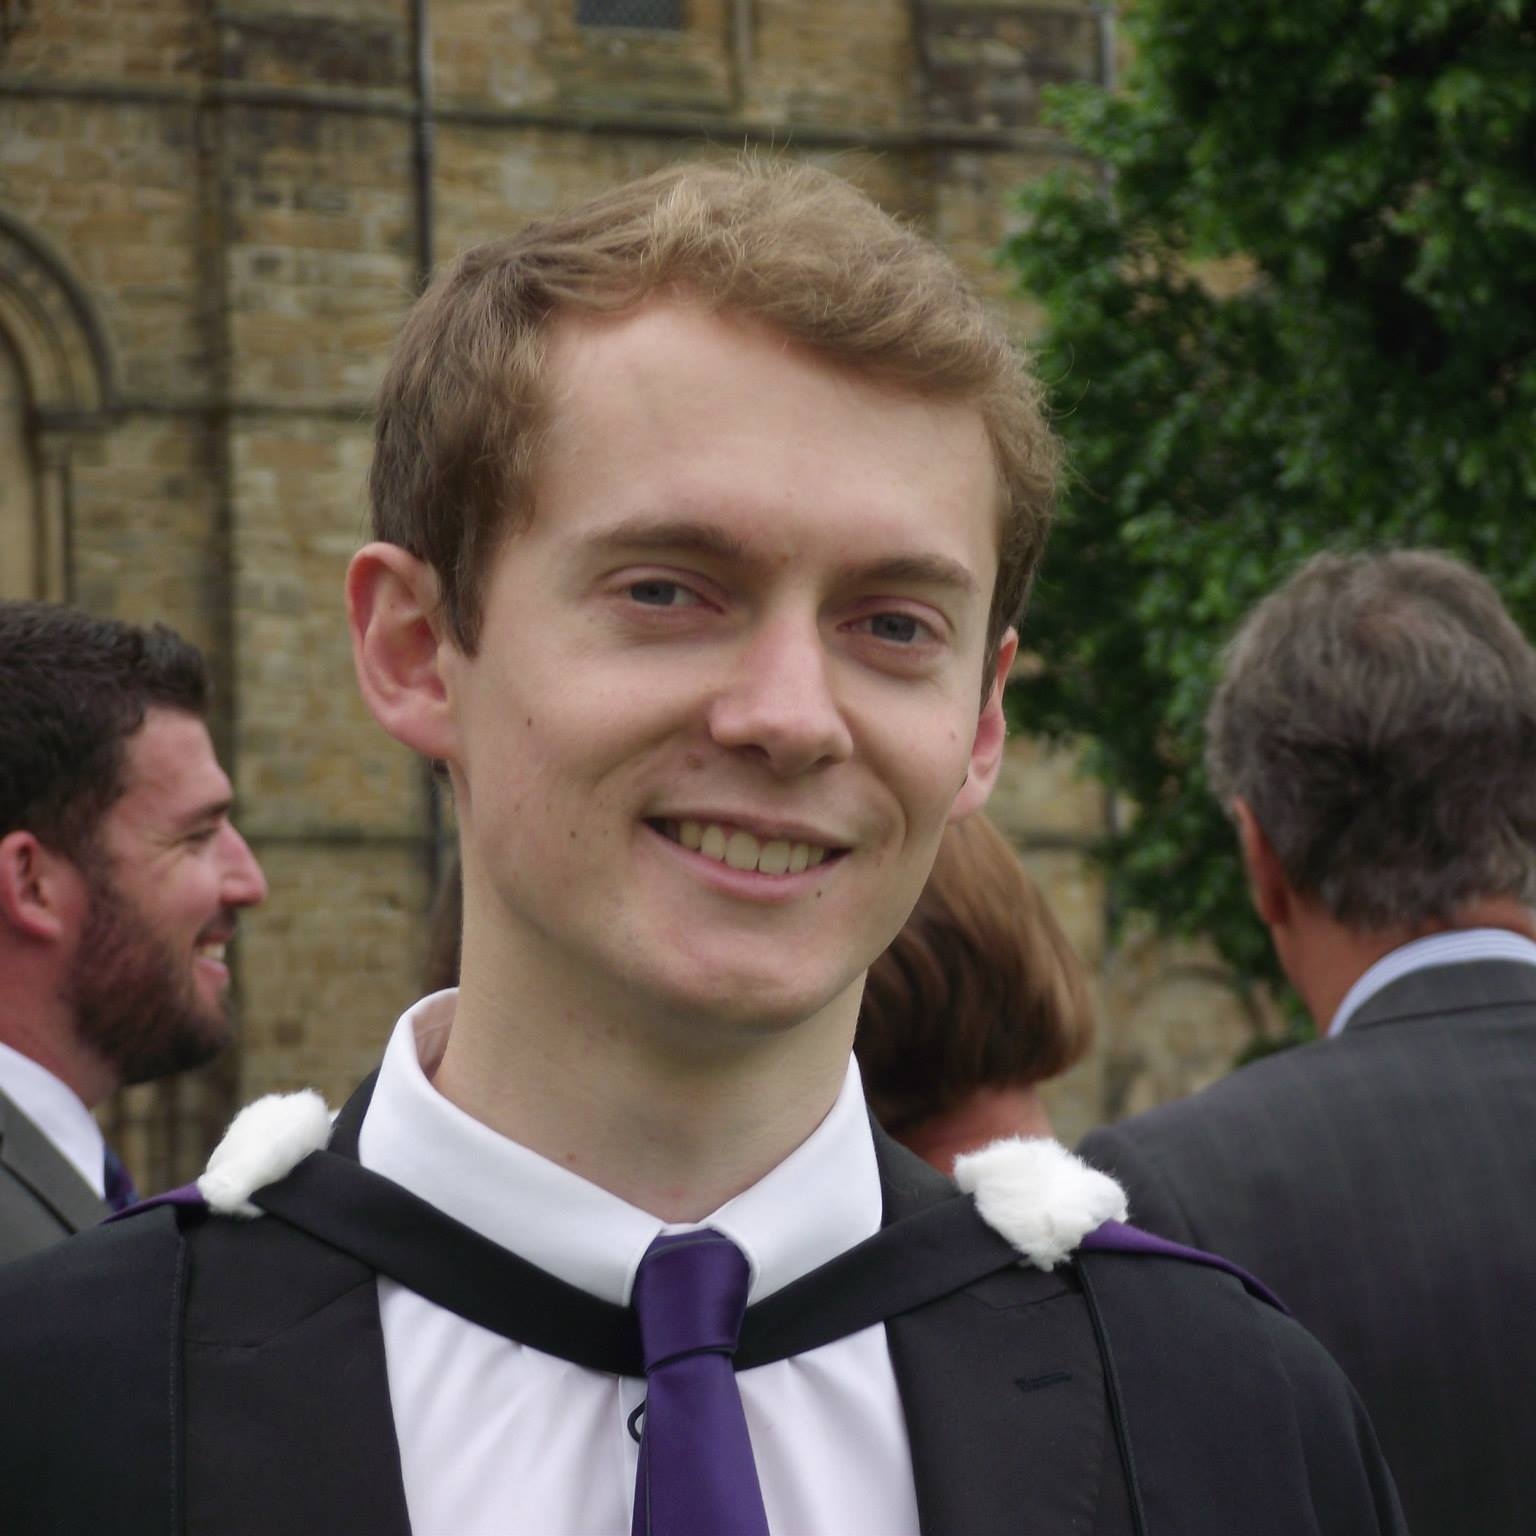
\includegraphics[width=\columnwidth]{graduation.jpg}
	\vspace{-8cm}
\end{figure}

\begin{flushright}\small
	\href{adamc@roe.ac.uk}{adamc@roe.ac.uk}  \\
	\SmallSep
	\href{https://www.roe.ac.uk/~adamc}{roe.ac.uk/$\sim$adamc} \\
	\SmallSep
	\href{https://www.github.com/ACCarnall}{github.com/ACCarnall} \\
\end{flushright}\normalsize
\framebreak


% Right frame
\Huge\bfseries {\color{RoyalBlue} Adam Carnall} \\
%\Large\bfseries Astrophysics PhD Student \\
\normalsize\normalfont

Astrophysics PhD student working on galaxy spectral modelling and fitting.

\Sep

\CVSection{Interests and Skills}

 - Galaxy formation and evolution\\
 - Bayesian statistical analysis\\
 - Software development in Python\\
 - Machine learning and optimisation techniques\\
 - I also climb mountains in my spare time!

\Sep

\CVSection{Education}
\CVItem{2015 -- present: \textcolor{black}{PhD Astrophysics, Royal Observatory Edinburgh}}\\
 - Thesis title: The star-formation histories of quiescent galaxies \\
 - Supervisors: Prof. Ross J. McLure and Prof. James S. Dunlop
 
 \SmallSep

\CVItem{2011 -- 15: \textcolor{black}{MPhys Physics and Astronomy, Durham University}}\\
 - Graduated with first class honours: final mark 82\%\\
 - Final year project: A new search for high redshift quasars\\
 - Supervisor: Prof. Tom Shanks
 
 \SmallSep
 
\CVItem{2007 -- 11: \textcolor{black}{GCSEs + A-levels, Thirsk School and Sixth Form College}}\\
 - A-levels: A*A*A*A* in Physics, Chemistry, Maths and Further Maths\\
 - AS-levels: AA in Geography and General Studies\\
 - GCSEs: Eight A* grades and two A grades
 
\Sep

\CVSection{First Authored Publications}

\textbf{\color{RoyalBlue}2018: \textcolor{black}{The VANDELS Survey: The star-formation histories of massive quiescent galaxies at 1.0 \textless\ z \textless\ 1.3}} - in preparation, to be submitted to MNRAS

\SmallSep

\textbf{\color{RoyalBlue}2018: \textcolor{black}{How well-motivated are parametric star-formation history models?}} - in preparation, to be submitted to ApJ

\SmallSep

\textbf{\color{RoyalBlue}2018: \textcolor{black}{Inferring the star-formation histories of massive quiescent galaxies with BAGPIPES}} - {\color{RoyalBlue}\href{https://academic.oup.com/mnras/article-abstract/480/4/4379/5068189}{MNRAS 480, 4379}}

\SmallSep

\textbf{\color{RoyalBlue}2017: \textcolor{black}{SpectRes: A fast spectral resampling tool in Python}} - {\color{RoyalBlue}\href{https://arxiv.org/abs/1705.05165}{arXiv:1705.05165}}

\SmallSep

\textbf{\color{RoyalBlue}2015: \textcolor{black}{Two bright z \textgreater\ 6 quasars from VST ATLAS and a new method of optical plus mid-infrared colour selection}} - {\color{RoyalBlue}\href{https://academic.oup.com/mnrasl/article-abstract/451/1/L16/954689?redirectedFrom=PDF}{MNRAS Letters 451, 16}}

\Sep

\CVSection{Coauthored Publications}

\textbf{\color{RoyalBlue}2018: \textcolor{black}{The VANDELS ESO public spectroscopic survey}} - \textit{R. J. McLure et al. (tenth author)} - {\color{RoyalBlue}\href{https://academic.oup.com/mnras/article-abstract/479/1/25/4995916}{MNRAS 479, 25}}

\SmallSep

\textbf{\color{RoyalBlue}2018: \textcolor{black}{Two more, bright, z \textgreater\ 6 quasars from VST ATLAS and WISE}} - \textit{B. Chehade et al. (second author)} - {\color{RoyalBlue}\href{https://academic.oup.com/mnras/article-abstract/478/2/1649/4944228}{MNRAS 478, 1649}}

\SmallSep

\textbf{\color{RoyalBlue}2018: \textcolor{black}{The VANDELS ESO public spectroscopic survey: observations and first data release}} - \textit{L. Pentericci et al. (tenth author)} - {\color{RoyalBlue}\href{https://www.aanda.org/component/article?access=doi&doi=10.1051/0004-6361/201833047}{A\&A Accepted}}

\SmallSep

\textbf{\color{RoyalBlue}2017: \textcolor{black}{The VANDELS survey: Dust attenuation in star-forming galaxies at z=3-4}} - \textit{F. Cullen et al. (sixth author)} - {\color{RoyalBlue}\href{https://academic.oup.com/mnras/article-abstract/476/3/3218/4898075}{MNRAS 476, 3218}}\\

\clearpage
\framebreak
\framebreak

\CVSection{Software Development}

\CVItem{\textcolor{black}{BAGPIPES: Bayesian Analysis of Galaxies for Physical Inference and Parameter EStimation -} {\color{RoyalBlue}\href{https://bagpipes.readthedocs.io}{bagpipes.readthedocs.io}}}

 \SmallSep

\CVItem{\textcolor{black}{SpectRes: Spectral Resampling -} {\color{RoyalBlue}\href{https://spectres.readthedocs.io}{spectres.readthedocs.io}}}

\Sep

\CVSection{Conference Talks}

\CVItem{2018: \textcolor{black}{IAU Symposium 341: Challenges in Panchromatic Galaxy Modelling with Next Generation Facilities, Osaka}}\\
 - Talk: Advanced panchromatic spectral modelling and fitting with BAGPIPES
 
 \SmallSep
 
\CVItem{2018: \textcolor{black}{The Art of Measuring Galaxy Physical Parameters, UC Riverside}}\\
 - Invited talk: Review of star-formation and chemical-enrichment histories\\
 - Invited talk: Advanced spectral modelling with BAGPIPES 
 
 \SmallSep

\CVItem{2018: \textcolor{black}{The Growth of Galaxies in the Early Universe IV, Sesto}}\\
 - Talk: Advanced spectral modelling with BAGPIPES
 
 \SmallSep

\CVItem{2018: \textcolor{black}{Durham Edinburgh Extragalactic Conference XIV, Durham}}\\
 - Talk: Inferring the SFHs of massive quiescent galaxies with BAGPIPES 
 
 \SmallSep

\CVItem{2017: \textcolor{black}{Royal Society of Edinburgh Cormack Meeting}}\\
 - Talk: Understanding galaxy quenching with BAGPIPES
 
  \SmallSep

\CVItem{2017: \textcolor{black}{Advances in Galaxy Evolution with Surveys, Ringberg Castle}}\\
 - Invited talk: Understanding galaxy evolution with VANDELS
 
\Sep

\CVSection{Awards and Scholarships}

\CVItem{2018: \textcolor{black}{Scottish Universities Physics Alliance PECRE Bursary}}\\
 - Funding for five week visit to the Harvard-Smithsonian Center for Astrophysics 
 
\SmallSep

\CVItem{2015: \textcolor{black}{Durham University J. A. Chalmers Prize in Experimental Physics}}\\
 - Awarded for best final year research project
 
\SmallSep
 
\CVItem{2015: \textcolor{black}{Durham University Summer Research Placement Bursary}}\\
 - Funded six week summer research project supervised by Prof. T. Shanks
 
\SmallSep

\CVItem{2014: \textcolor{black}{Institute of Physics Top 50 Award: Southampton University}}\\
 - Funded eight week research project supervised by Dr. D. Altamirano
 
\SmallSep

\CVItem{2013: \textcolor{black}{Oxford University Summer Research Programme}}\\
 - Funded eight week summer research project supervised by Dr. R. Houghton
 
\SmallSep

\CVItem{2013: \textcolor{black}{Leicester University SURE Bursary}}\\
 - Funded six week summer research project supervised by Prof. A. Blain

\Sep

\CVSection{Teaching and Supervision}

\CVItem{2018: \textcolor{black}{Edinburgh University Physics Summer Scholarship}}\\
 - Supervised undergraduate student Jamie Yellen for 8 week project\\
 - Project title: Advanced Bayesian methods for galaxy spectral fitting
 
 \SmallSep
 
\CVItem{2017: \textcolor{black}{Royal Society of Edinburgh Cormack Research Scholarship}}\\
 - Supervised undergraduate student Joe Cairns for 6 week project\\
 - Project title: SCUBA-diving in the deep universe: The origins of massive galaxies
 
\SmallSep

\CVItem{2015-present: \textcolor{black}{Edinburgh University Teaching Assistant}}\\
 - I teach tutorials and labs for a variety of undergraduate courses

\clearpage
\framebreak
\framebreak

\CVSection{Outreach, Voluntary Activities and Hobbies}

\CVItem{2018: \textcolor{black}{Royal Observatory Edinburgh Doors Open Day Volunteer}}\\
 - Organised stall exhibiting ROE research involving spectroscopic surveys
 
 \SmallSep
 
\CVItem{2017: \textcolor{black}{Royal Observatory Edinburgh Christmas Ceilidh Organiser}}

\SmallSep

\CVItem{2017 -- Present: \textcolor{black}{Edinburgh Physics Postgraduate Forum member}}\\
 - Member of staff-student liason committee responsible for delivering student feedback and organising department-wide social events

\SmallSep

\CVItem{2017: \textcolor{black}{Royal Observatory Edinburgh Doors Open Day Volunteer}}\\
 - Outreach talk: Astronomical archaeology: how do galaxies form?
 
 \SmallSep
 
\CVItem{2017: \textcolor{black}{Edinburgh University Physics Department Firbush Organiser}}\\
 - Organised a week-long outdoor activities trip for PhD students in physics
 
 \SmallSep

\CVItem{2015 -- present: \textcolor{black}{Edinburgh University Hillwalking Club}}\\
- Treasurer 2016-17: Managed a budget of \pounds40,000 \\
- I drive minibuses and lead walks on weekend trips to the highlands

\SmallSep

\CVItem{2013 -- 2015: \textcolor{black}{Durham University Humanist Students Society}}\\
 - President 2014 -- 15: Organised speaker events, socials and campaigns\\
 - Treasurer 2013 -- 14: Managed a budget of \pounds2000
 
 \SmallSep
 
\CVItem{2012 -- 15: \textcolor{black}{Durham University Cross Country Club Member}}





\end{document}